%%%%%%%%%%%%%%%%%%%%%%%%%%%%%%%%%%%%
% Header                           %
%%%%%%%%%%%%%%%%%%%%%%%%%%%%%%%%%%%%
% 
% Revisions: 2017-04-10 Martin Rädel <martin.raedel@dlr.de>
%                       Initial draft
%               
% Contact:   Martin Rädel,  martin.raedel@dlr.de
%            DLR Composite Structures and Adaptive Systems
%          
%                                 __/|__
%                                /_/_/_/  
%            www.dlr.de/fa/en      |/ DLR
% 
%%%%%%%%%%%%%%%%%%%%%%%%%%%%%%%%%%%%
% Content                          %
%%%%%%%%%%%%%%%%%%%%%%%%%%%%%%%%%%%%

\leveldown{Download}

\leveldown{Download the official release}
\label{sec:Install:Peridigm:Download}

The current official release of \marktool{\toolname} can be obtained from the download section of

\href{\tooladdress}{\tooladdress}

The download needs a short registration with a valid email-address. Download the \verb+tgz+ file of your preferred \marktool{\toolname} version to \verb+$DOWNLOAD_DIR+. Unpack the archive:

\begingroup
\lstset{breaklines=true}
\begin{code}
cd $DOWNLOAD_DIR
tar xvfz Peridigm_1.4.1.tgz
\end{code}
\endgroup

\levelstay{Download the latest master version from \texorpdfstring{\protect\marktool{\githubname{}}}{\githubname{}}}

The \marktool{\toolname} repository is available from \marktool{\githubname} and can be downloaded from:

\href{\toolrepoaddress}{\toolrepoaddress}

To obtain the latest master release go to that homepage and select the \textit{master} branch in the top left and click on \textit{Download zip} in the top right corner as shown by the red rectangles in \autoref{fig:Peridigm_GitHubRepository_Homepage_Master} or click this \href{\toolrepoaddresszip}{link}.

\begin{figure}[htbp]
\centering
 \begin{tikzpicture}
   % External figure
   \node[anchor=south west,inner sep=0] (image) at (0,0){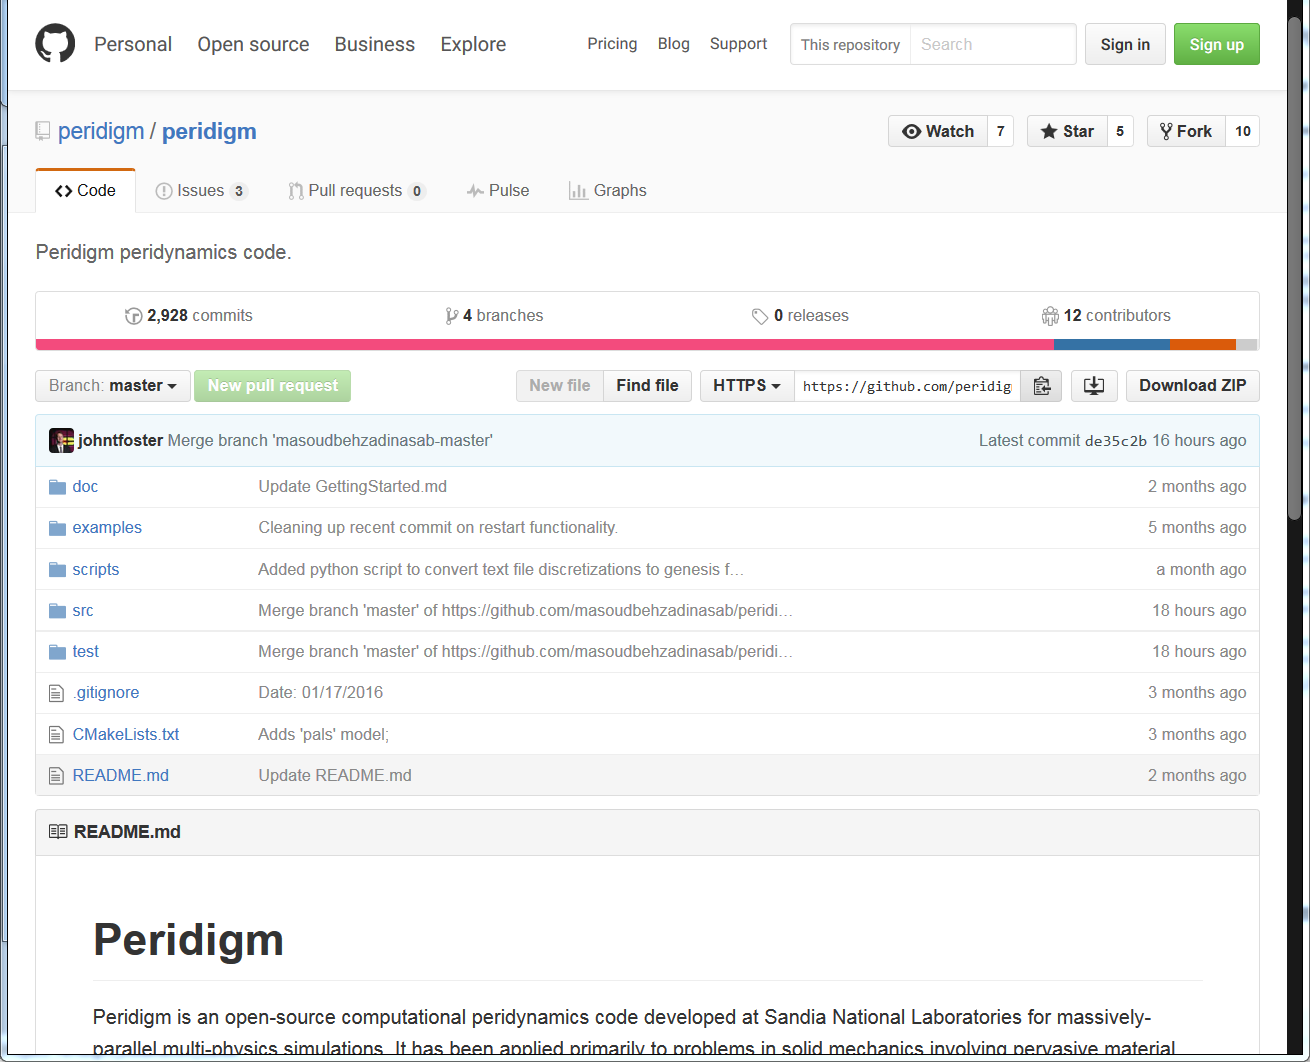
\includegraphics[width=0.95\linewidth]{Figures/Peridigm_GitHubRepository_Homepage_Master}};
   % Figure scope
   \begin{scope}[
     x={(image.south east)},
     y={(image.north west)},
   ]
     % Red rectangle Master
     \draw[red,ultra thick,rounded corners] (0.02,0.615) rectangle (0.1525,0.6575);
     % Red rectangle Download
     \draw[red,ultra thick,rounded corners] (0.8535,0.615) rectangle (0.9675,0.6575);
     % Help grid and labels
     %\pic{myimagegrid};
   \end{scope}
 \end{tikzpicture}
 \caption{\protect\marktool{\toolname} \protect\marktool{\githubname} repository screenshot}
 \label{fig:Peridigm_GitHubRepository_Homepage_Master}
\end{figure}

Unpack the archive:

\begingroup
\lstset{breaklines=true}
\begin{code}
cd $DOWNLOAD_DIR
unzip peridigm-master.zip
mv peridigm-master Peridigm-1.4.1-Source
\end{code}
\endgroup

\levelstay{Checkout the latest version from \texorpdfstring{\protect\marktool{\githubname{}}}{\githubname{}}}

\leveldown{With svn}

Use \marktool{kdesvn} to checkout the latest version. Checkout

\href{https://github.com/peridigm/peridigm.git/trunk}{https://github.com/peridigm/peridigm.git/trunk}

\levelstay{With git}

Use \marktool{git} on the cluster:

\begingroup
\lstset{breaklines=true}
\begin{code}
git clone https://github.com/peridigm/peridigm.git
\end{code}
\endgroup

\levelmultiup{Compiling \& installation}{2}

\marktool{\toolname} utilizes the \marktool{\cmakename} build system. It is recommended that Makefiles be created by running \verb+cmake+ from the command line, as opposed to using the \verb+ccmake+ GUI.

The installation here is described for the then official \marktool{\toolname} version 1.4.1. The steps for version 1.5 are identical besides the changes in folder names.

\marktool{\toolname} does not allow the use of the directory with the source-files for the further progress of the installation. Therefore, create a new folder

\begin{code}
mkdir Peridigm-1.4.1
\end{code}

and copy the file from section \ref{sec:Build-script_Peridigm} to the new folder. Change the lines for the library paths and the \marktool{\toolnameshort}-source-directory (last line) if necessary.

In order to use the script make it executable as described in section \ref{sec:Build-script_Executable}. Open a terminal as root, change directory to the created path and execute it with

\begin{code}
./cmake_peridigm.cmake > cmakeopts.log 2>&1
\end{code}

Once \marktool{\toolname} has been successfully configured, it can be compiled and installed as follows:

\begin{code}
make -j 4
make install
\end{code}

The default location for the created binary is \verb+/usr/local/bin/+. In case you want to create the binary at a different location add the following line to the script from section \ref{sec:Build-script_Peridigm}

\begin{code}
-D CMAKE_INSTALL_PREFIX=/PATH/TO/DESTINATION
\end{code}

After installation make sure to change permissions of the installation directory for the necessary users and groups.

\levelstay{After building and installing}

\cite{PeridigmUserGuide100} recommends to run \verb+ctest+ in your build directory after building and installing \marktool[\tooladdress]{\toolname} to run all tests and confirm that you have a clean build. Alternatively, \marktool[\tooladdress]{\toolname} offers an own test suite which is used here.

To be able to execute the test you first have to temporarily change the source and installation folder owner. Thus perform the following commands before executing the test.

\begin{code}
chown -R $USERNAME:$GROUPNAME Peridigm-1.4.1
chown -R $USERNAME:$GROUPNAME Peridigm-1.4.1-Source
\end{code}

Before starting the test-suite as a normal user, open a new shell or use an existing one and re-register your username to load the current state of the \verb+.bashrc+-file:

\begin{code}
su - $USERNAME
\end{code}

The \marktool[\tooladdress]{\toolname} test suite is then run from the terminal as non-root user as follows:

\begin{code}
make test
\end{code}

Remember to revert the modifications to the \marktool{\toolname} directory ownership after it is assured that all tests are passed with:

\begin{code}
chown -R root:root Peridigm-1.4.1
chown -R root:root Peridigm-1.4.1-Source
\end{code}

\levelstay{Install a local version on the cluster}

\begin{enumerate}[noitemsep]
  \item Login to the STM cluster and move to a directory of your convenience
  \item Clone your local \toolname{} version from GitHub with \verb+git clone+ or download the master zip-file and unpack, see section \ref{sec:Install:Peridigm:Download}
  \item Allocate cluster-node exclusively for building
\begin{code}
salloc --exclusive
\end{code}
  \item Load build and library environment
\begin{code}
. /cluster/software/slurm/etc/env.d/mpibuild.sh 
. /cluster/software/slurm/etc/env.d/peridigm.sh
\end{code}
  %\item Change directory to the local \toolname{} directory
\item Change directory to the folder, where the unpacked \toolname{} source folder is located
\begin{code}
cd ~/src/peridigm
\end{code}
  \item Create a build-directory and go to the new directory
\begin{code}
mkdir peridigm-build
cd peridigm-build
\end{code}
  \item Save the following lines in the file \texttt{cmake\_peridigm.cmake}. Change the path in the code to the correct location.
\begingroup
\lstset{breaklines=true}
\begin{code}
cmake \
-D CMAKE_BUILD_TYPE:STRING=Release \
-D CMAKE_INSTALL_PREFIX=/home/USER/peridigm-build \
-D CMAKE_CXX_FLAGS:STRING='-O2 -Wall -std=c++11 -pedantic -Wno-long-long -ftrapv -Wno-deprecated' \
/home/USER/peridigm-master
\end{code}
\endgroup
  \item Call \cmakename{} via terminal with the given code:
\begingroup
\lstset{breaklines=true}
\begin{code}
./cmake_peridigm.cmake
\end{code}
\endgroup
  \item Make
\begin{code}
make -j 8
\end{code}
  \item Test
\begin{code}
make test
\end{code}
  \item Create the executable 
\begin{code}
make install
\end{code}
  \item Exit salloc shell
\begin{code}
exit
\end{code}
  \item The executable is now located at \verb+~/src/peridigm/peridigm-build/bin+
  \item For how to execute the local version using the cluster queuing-system look at the \toolname{} User Guide
\end{enumerate}

A complete script for cloning \toolname{} from GitHub, compiling and installing on the cluster can be found in \autoref{sec:Build-script_Peridigm:Cluster}.

\levelstay{Use of \texorpdfstring{\protect\marktool{Docker}}{Docker}}

\href{http://johntfoster.github.io/posts/peridigm-without-building-via-Docker.html}{http://johntfoster.github.io/posts/peridigm-without-building-via-Docker.html} 